\documentclass[12pt, a4paper]{article}

\usepackage[slovak]{babel}
\usepackage[utf8]{inputenc}
\usepackage[T1]{fontenc}
\usepackage{geometry}
\usepackage{hyperref}
\usepackage{setspace}
\usepackage{subcaption}
\usepackage{afterpage}
\usepackage{graphicx}
\usepackage{csquotes}
\usepackage{longtable}
\usepackage{pdfpages}
\usepackage{expl3}

% Dots in TOC
\usepackage{tocloft}
\renewcommand{\cftsecleader}{\cftdotfill{\cftdotsep}}


\setstretch{1.5}
\widowpenalty10000
\clubpenalty10000
\newsavebox\shield
\usepackage{titlesec}

\usepackage[style=iso-numeric,backend=biber]{biblatex}
\addbibresource{references.bib}
%\AtBeginBibliography{\small}

\geometry{
	a4paper,
	top=2cm,
	left=3cm,
	right=2.5cm,
	bottom=2.5cm
}

\begin{document}
\begin{titlepage}
{\centering
    {\Large Slovenská technická univerzita v Bratislave}\par
    {\Large Fakulta informatiky a informačných technológií}\par
    \vspace{\medskipamount}
    \vfill
    \LARGE \textbf{Inteligentné osvetlenie pracovného stola} \\
    \vspace{0.7\bigskipamount}
    {\Large Semestrálny projekt}\par
    \vfill
}
\normalsize    
\begin{flushleft}
\textbf{Autor:} Bc. Miroslav Hájek \\
\textbf{Študijný program:} Inteligentné softvérové systémy \\
\textbf{Ročník:} 1. \\
\textbf{Predmet:} Vnorené systémy \\
\textbf{Akademický rok:} 2022 / 2023 \\
\end{flushleft}
\end{titlepage}

\thispagestyle{empty}
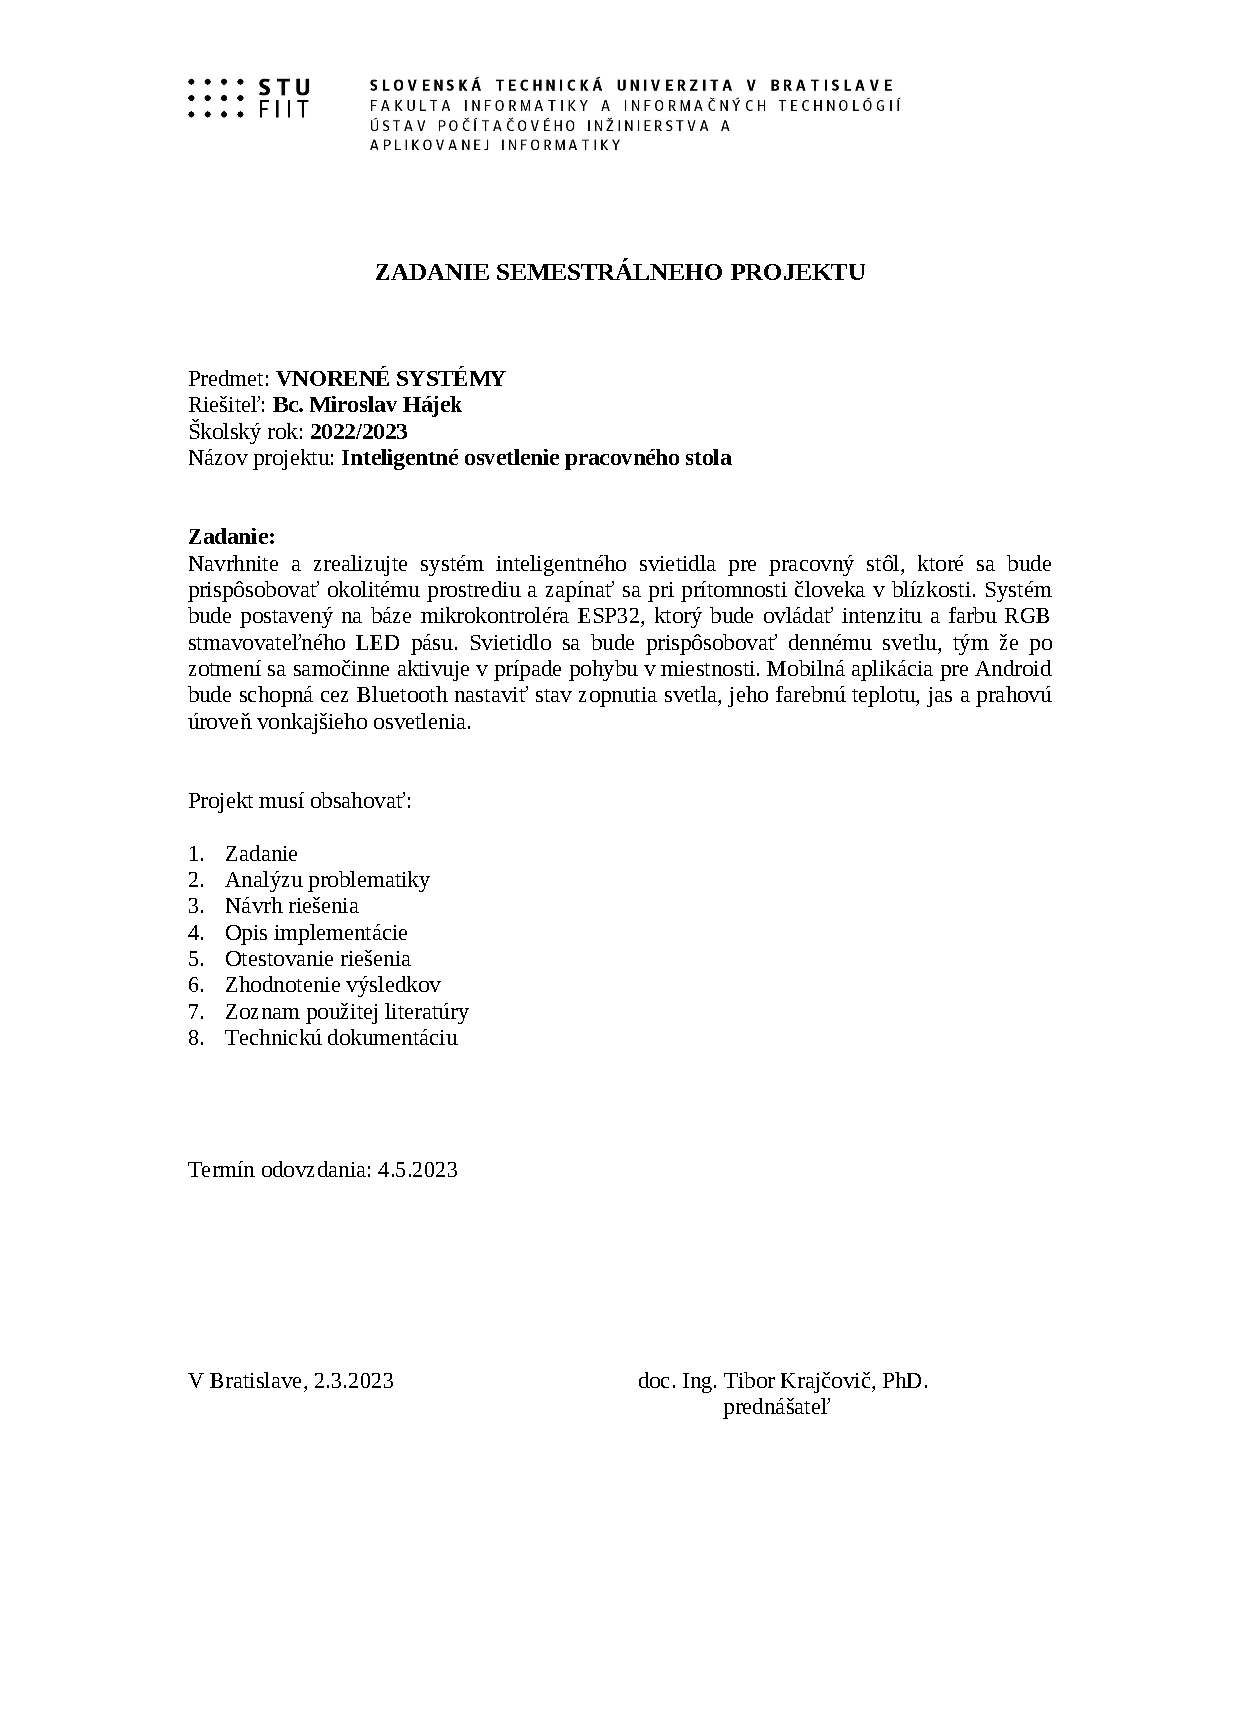
\includepdf[pages=-, scale=1]{zadanie}

\pagenumbering{gobble}
\tableofcontents
\newpage

\pagenumbering{arabic}
\setcounter{page}{1}

\section{Analýza problematiky}
% Moduly a ich cena, driver
Dôvod pre takéto svetlo: Motivácia
Požiadavky

\subsubsection{MCU, Senzory, Akčné členy}
Zdôvodnenie každého prvku, alternatívy
\begin{itemize}
\item ESP32 Lolin D32 - 3,3 V, Dostatok pamäte, Bluetooth vstataný (nedá sa použiť), FreeRTOS (viaceré tasky), ESP-IDF (dobrú podporu)
\item HC-05 Bluetooth modul - komunikácia cez UART na predvolených 9600 Baud, popis pinov, 
\item RGB LED pásik 14,4W/m 12V bez krytia IP20 1m - výkonový pásik, trojica v sérii RGB LED-iek v úsekoch 10 cm, rezistory. 
\item PIR-SB312 (Olimex) 10x8mm - Detekcia pohybu (do 3,6V, 10mA) 
\item WS-17146 TSL25911 Light Sensor  - Meranie vonkajšieho osvetlenia
\end{itemize}

\url{https://www.123led.sk/rgb-led-pasik-14-4w-m-bez-krytia/}
RGB LED pásik dokáže vytvoriť akúkoľvek farbu. Farby vznikajú miešaním červenej, zelenej a modrej.
Z výkonu 14,4W/m RGB pásik vyprodukuje až 550lm/m. Hustota LED diód je 60ks/m, opasok vďaka tomu svieti rovnomerne po celej svojej dĺžke. Tento pásik je potrebné nalepiť do hliníkovej lišty z dôvodu odvodu tepla z LED diód. Všetky naše pásky sú vybavené samolepiacou fóliou 3M 300LSE, ktorá skvele priľne k podkladu. Ten musí byť hladký a je potrebné ho pred lepením poriadne odmastiť.

\url{https://www.olimex.com/Products/Components/Sensors/PIR-SB312/}
    Static power consumption: <0.1mA; 
    Delay time: 2 seconds; 
    Block time: 2 seconds; 
    Trigger mode: repeatable; 
    Sensing range: <= 100 degrees cone angle, 3-5 meters
    Working temperature: -20 - + 85 ℃ 
    PCB Dimensions: 10mm x 8mm
    
  \url{https://www.waveshare.com/wiki/TSL25911_Light_Sensor}
  
  Light sensor: TSL25911FN
Communication interface: I2C (constant address: 0 x 29)
Effective range: 0~88000Lux


\subsubsection{Elektrické súčiastky}
\begin{itemize}
\item L7805CV Lineárny regulátor napätia 12V na 5V [0,40€] + DO3A chladič [€ 0,19]
\item NPN Tranzistor BD711 [€ 0,59] (3x + 3x DO1 chladič [€ 0,26])
\item Rezistory [2x 220 Ohm, 1x 330 Ohm]
\item LED zdroj (trafo) 12V 30W IP67 [€ 10,95]
\end{itemize}

\subsubsection{Mechanické súčiastky a prepoje}

\begin{itemize}
\item Univerzálny plošný spoj [€0,50]
\item Nástenný profil N3 biely + Opálový kryt 1m [€ 4,96]
\item Koncovka profilu N3 bílá [€0,41]
\item Flexo šnúra – 3m [€ 3,68]
\item Konektory: RGB LED pásik [€ 0,45], Micro USB-B [€0,50], DC konektor a zásuvka [€1,2]
\item Vypínač mezišnúrový [€ 0,41]
\end{itemize}
\newpage

\section{Návrh riešenia}
% Schémy
\begin{figure}
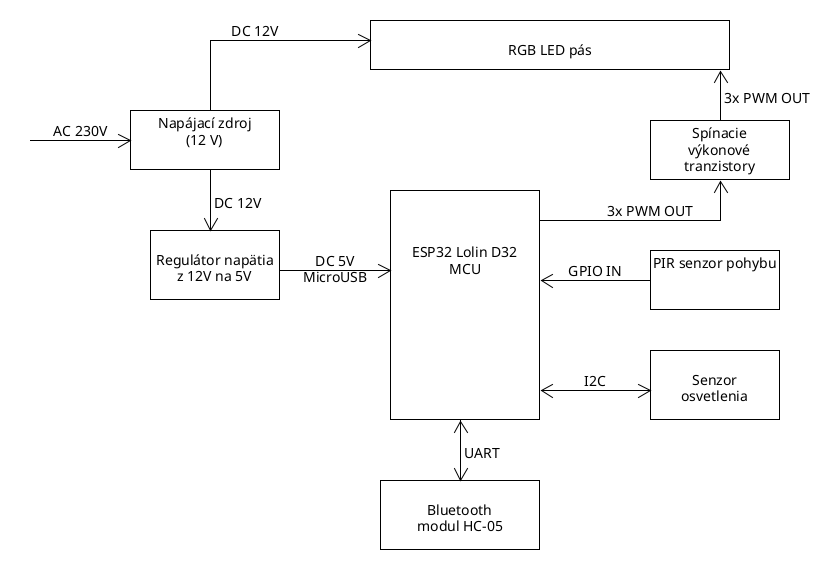
\includegraphics[width=\textwidth]{assets/block-diagram.png}
\end{figure}

\begin{figure}
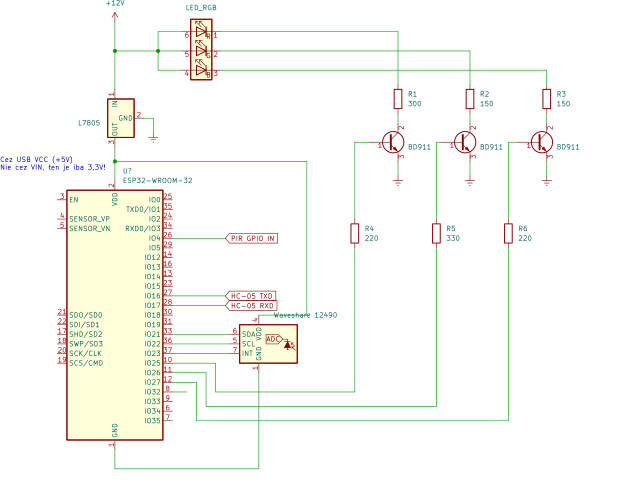
\includegraphics[width=\textwidth]{assets/electrical-schematics.png}
\end{figure}
% Wireframe mobilnej aplikácie

\subsection{Opis implementácie}
% Firmvér v ESP-IDF
% Softvér pre Android smartfón

\begin{figure}
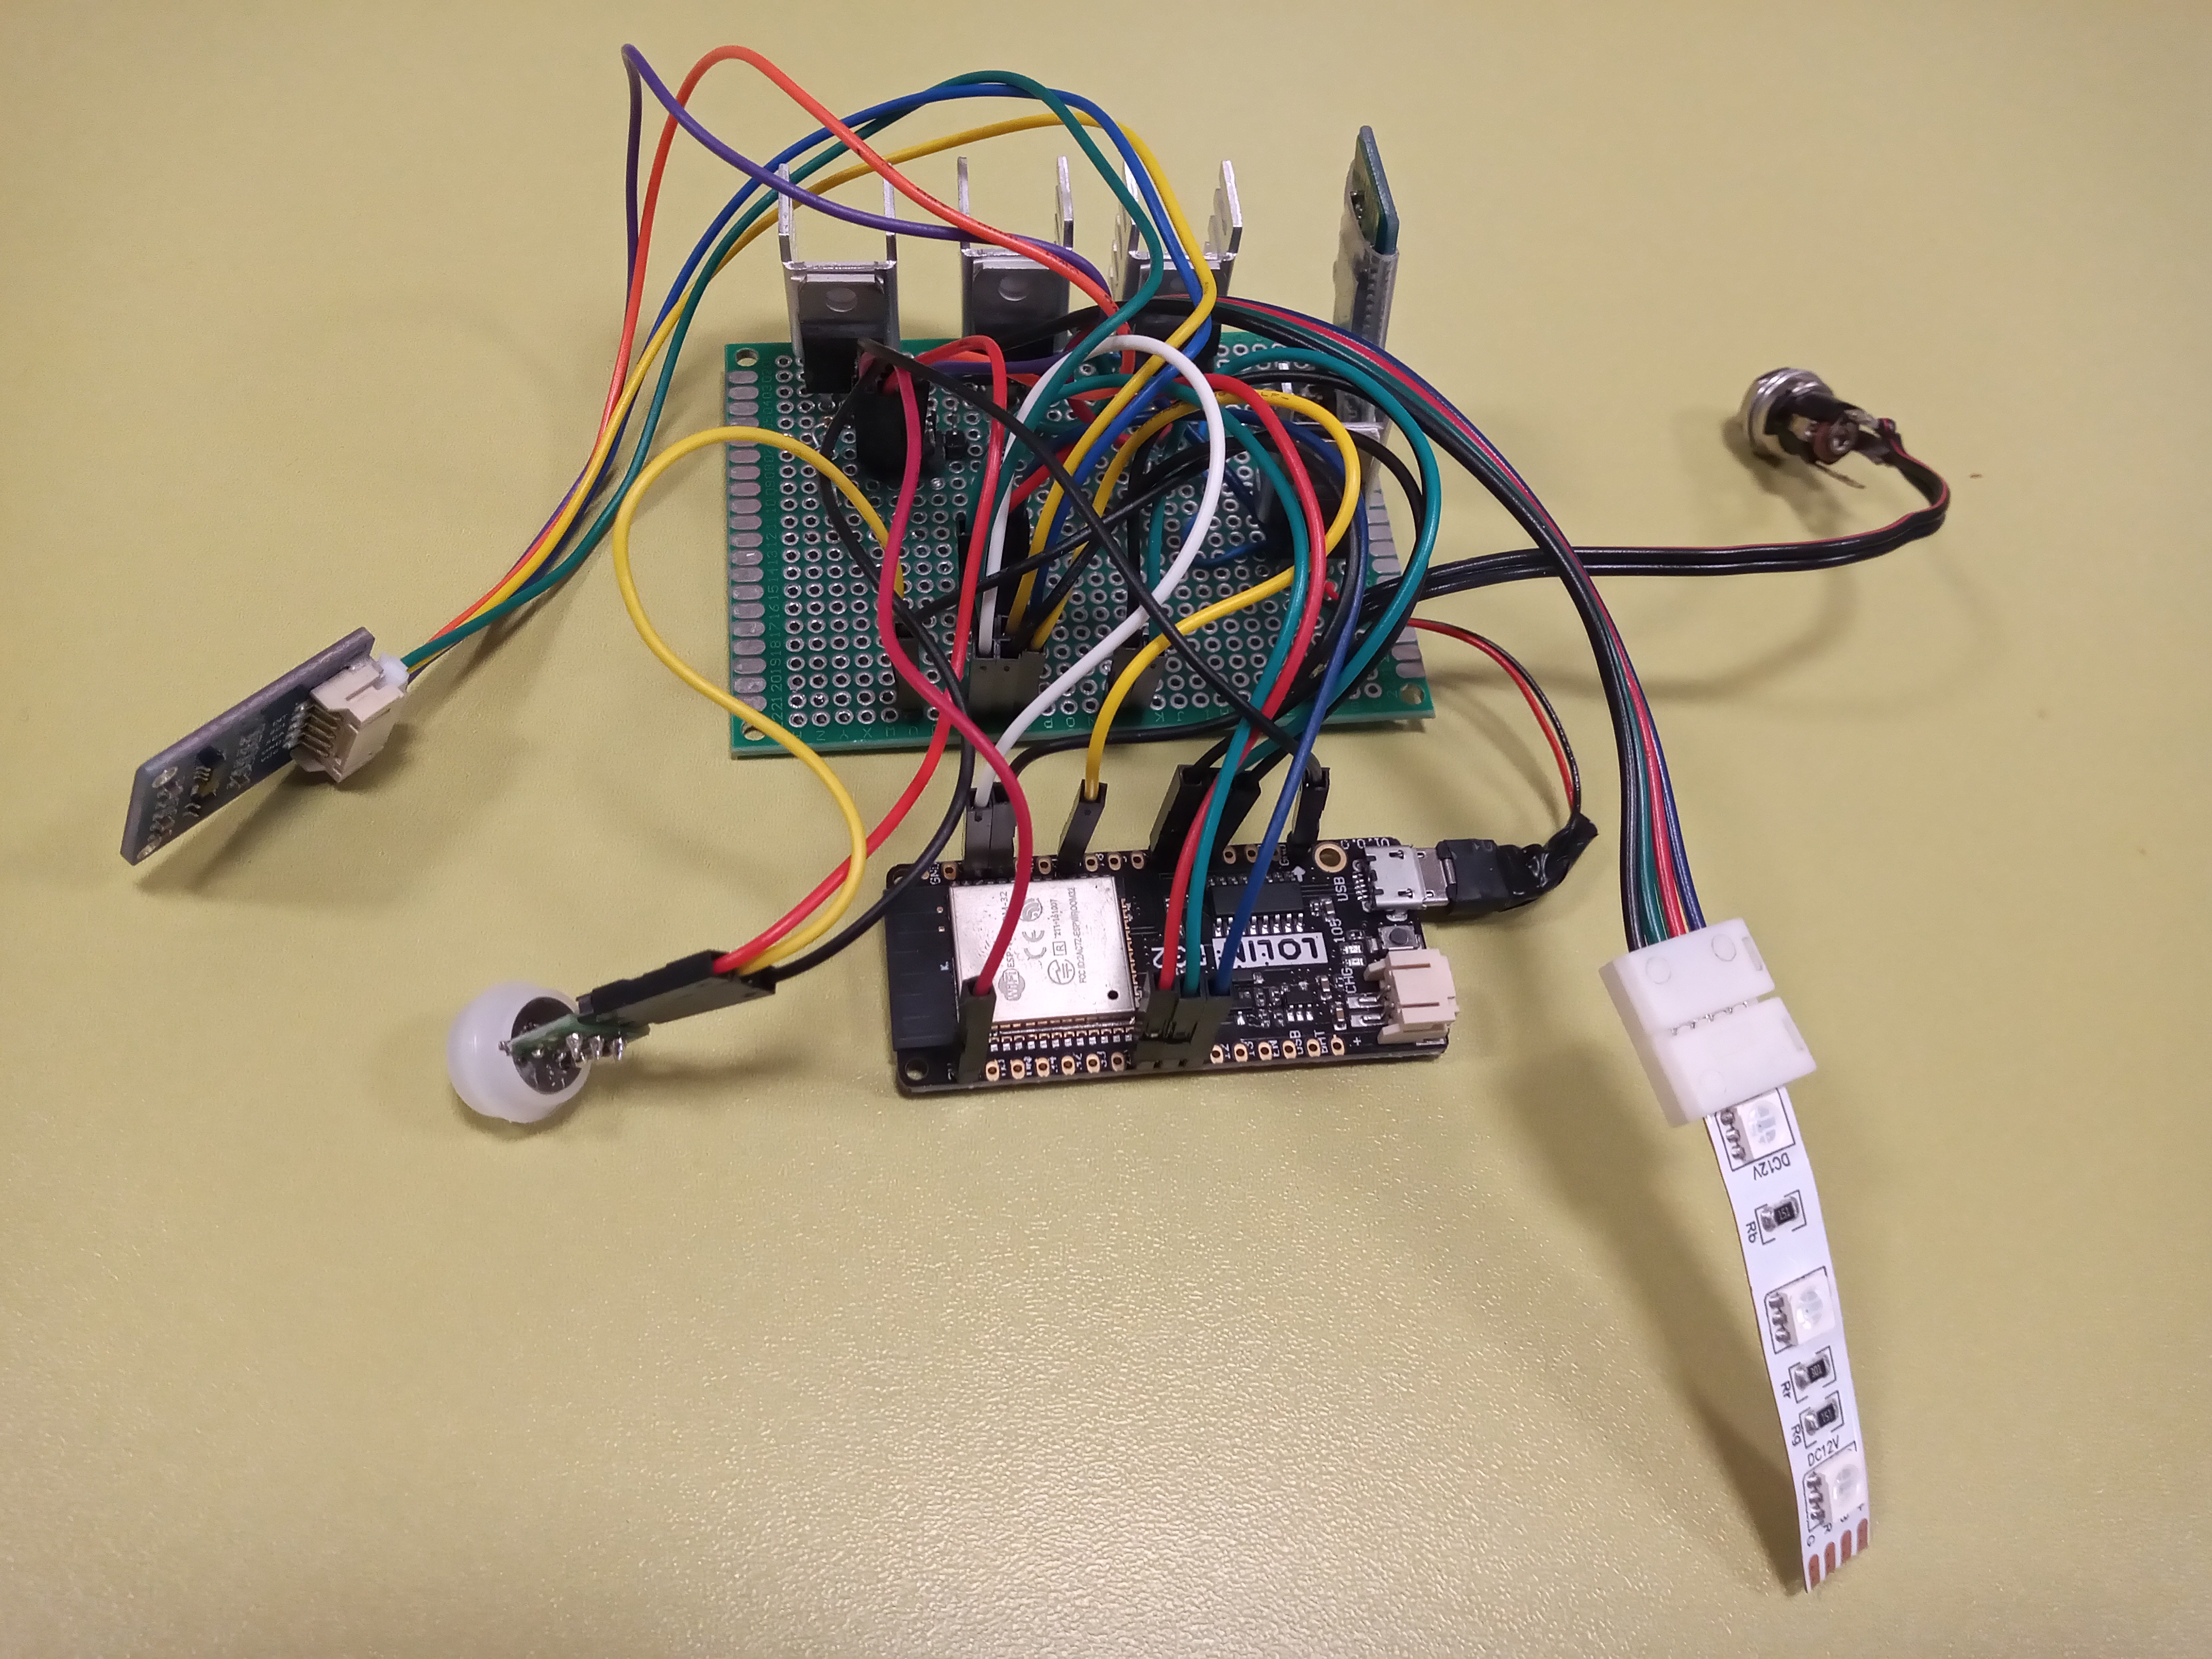
\includegraphics[width=\textwidth]{assets/prototype.jpg}
\end{figure}

\subsubsection{Spínanie svetla}
\begin{figure}
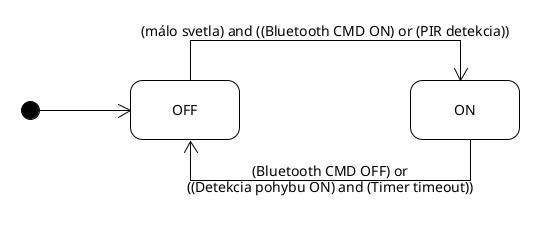
\includegraphics[width=\textwidth]{assets/light-states.png}
\end{figure}

\begin{figure}
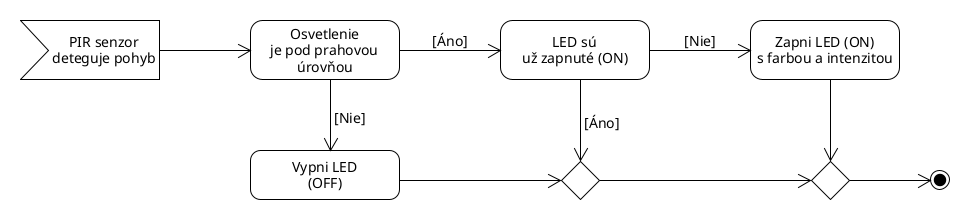
\includegraphics[width=\textwidth]{assets/pir-motion-detect.png}
\end{figure}

\subsubsection{Nastavenie farby a intenzity svietidla}
\begin{enumerate}
\item Kelvin ← Temperature
\item Kelvin →RGB (podľa regresného modelu)
\item RGB → HSV
\item V ←brightness
\item HSV→ RGB
\item PWM driver 8-bit OUT
\end{enumerate}

\subsubsection{Firmvér tasky}

% ESP-IDF - C kód a drivers 
% Android studio  (link na dokumentáciu)

\subsubsection{Mobilná aplikácia}
Obrazovka a popis fungovania

\subsection{Otestovanie riešenia}
% Testovacie scenáre - Akceptačné testy

% - 

\section{Zhodnotenie výsledkov}

\printbibliography[title={Literatúra}]
\url{https://tannerhelland.com/2012/09/18/convert-temperature-rgb-algorithm-code.html}
\newpage

\section{Technická dokumentácia}
% Štruktúra priečinkov
% Nahratie firmvéru
% Nahratie softvéru
% FW a SW: Moduly a funkcie

\end{document}